% ---------------------------------------------------------------------------------------
% Revised mechanistic interpretability section (condensed).
%
% Every number is reproduced by the scripts in the repository root:
%   behavioral_validation.py      --run-variance --run-steering --run-sanity --run-diagnostics
%   latent_steering.py            --run-checks --run-probe --run-clusters --run-steering
%   personalization_baselines.py  --n_users 200 [--item_context "item title"]
%   attribution_controls.py       --max_examples 60
% Results are written to results/*.json.
%
% Layout: figures and Tables 1-4 inline; Tables 5-6 under "APPENDIX CANDIDATES" at the end
% of this file, movable as-is because the prose quotes their key numbers.
%
% If more space is needed, in this order: (1) move the attribution subsection and its
% figure pair to the appendix, (2) drop Table~\ref{tab:variance_decomposition} and keep its
% three percentages in the prose, (3) make Table~\ref{tab:behavioral_validation} a
% single-column table showing only the State 3 columns.
%
% Changes to Table~\ref{tab:profile_perturbations} vs. the original: dropped the
% "Perturbation Type" column (folded into the State label) and the P(genre) > 0.9 figures,
% which the weak probe in this section no longer supports.
%
% TODO before submission: \ref{sec:results} is a placeholder for the results-section label.
% ---------------------------------------------------------------------------------------

\subsection{Mechanistic Interpretability}

To investigate how the fine-tuned recommender internalizes textual user profiles and responds to user interventions, we probe the final normalized layer of the transformer backbone using \texttt{nnsight}, extracting mean-pooled hidden activation vectors $\mathbf{h}_u \in \mathbb{R}^d$ for every user profile prompt (Appendix~\ref{sec:appendix_interp}). This captures the model's representation state immediately before classification.

\begin{figure*}[t]
    \centering
    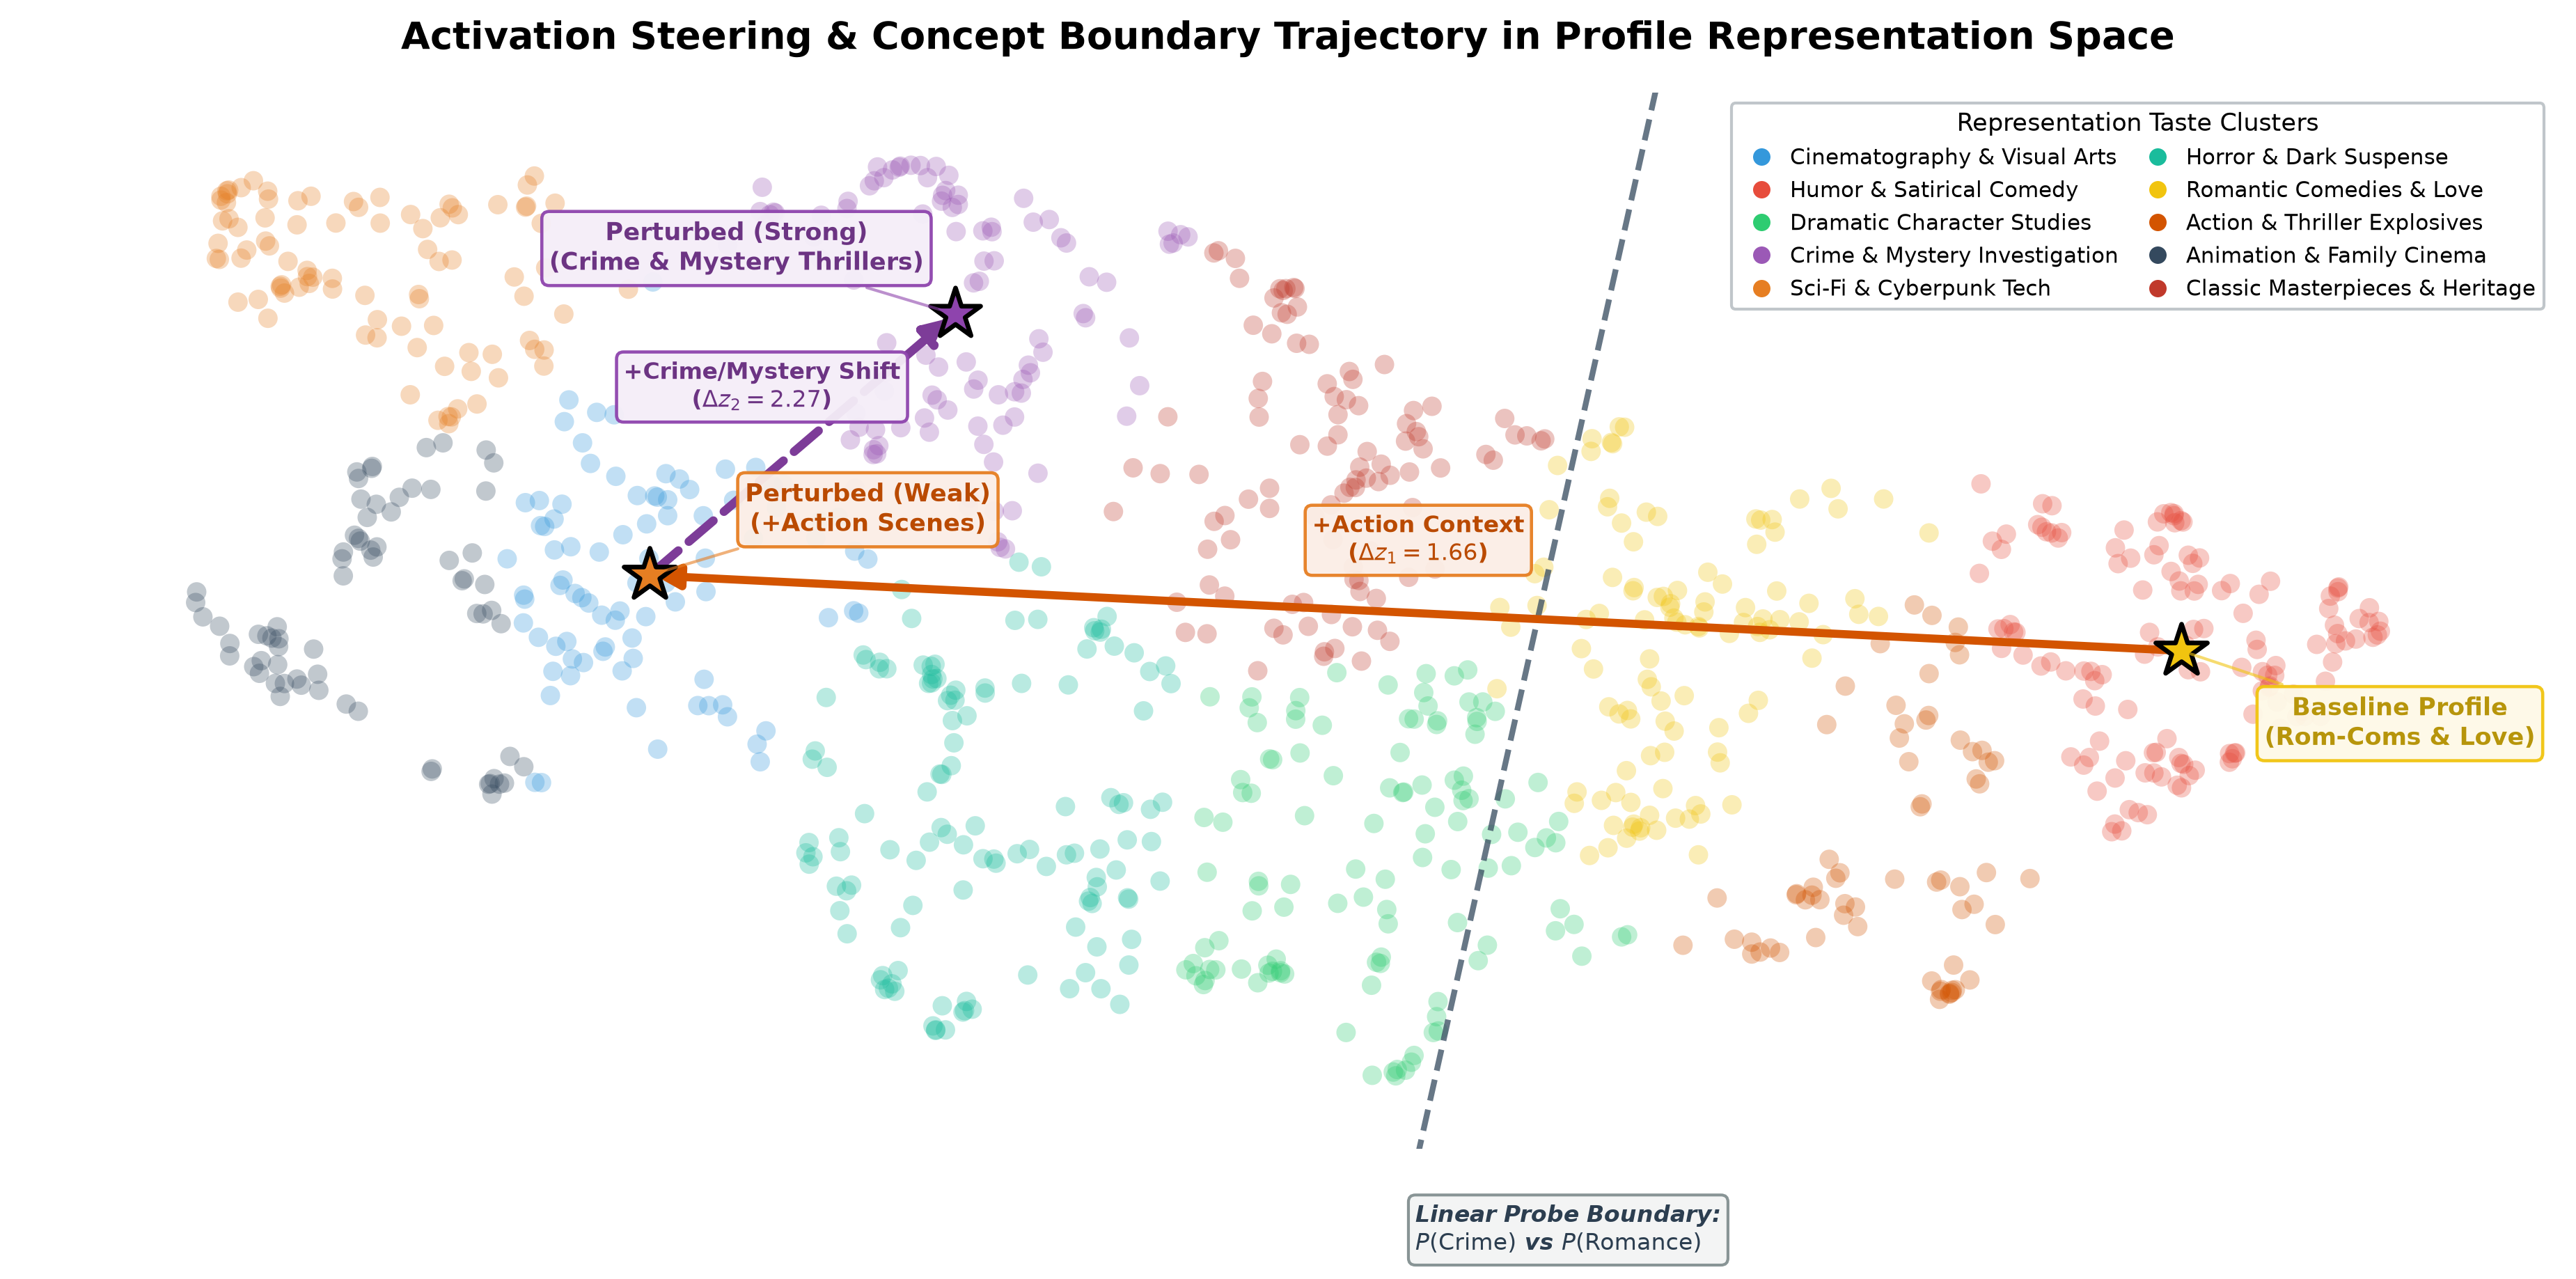
\includegraphics[width=\textwidth]{img/user_profile_perturbation.png}
    \caption{2D UMAP visualization of final layer normalization activations extracted via \texttt{nnsight}. Background point clouds are population-wide groupings of profile representations, color-coded and labeled by their most salient profile terms; these groupings track profile wording rather than user taste, agreeing with history-derived genre preference only at chance (adjusted Rand index $0.0008$, \S\ref{sec:repr_structure}). Trajectory vectors show the three counterfactual edits of Table~\ref{tab:profile_perturbations}, with a fitted linear probe boundary. The edits produce smooth, directional shifts in representation space; \S\ref{sec:repr_to_behavior} shows they do not carry through to predicted ratings or rankings.}
    \label{fig:perturbation}
\end{figure*}

\begin{table}[t]
    \centering
    \small
    \caption{Counterfactual profile perturbation states used in the trajectory analysis. Steering keywords added at each transition are in \textbf{bold}. The behavioral evaluation in \S\ref{sec:repr_to_behavior} uses length-matched paraphrases of these states at training-profile length (given in \texttt{behavioral\_validation.py}), since the strings below are shorter than any profile seen in fine-tuning.}
    \label{tab:profile_perturbations}
    \begin{tabular}{@{}lp{4.3cm}l@{}}
    \toprule
    \textbf{State} & \textbf{Natural-Language Profile Text} & \textbf{Target} \\
    \midrule
    1 (baseline) & \textit{``I like romantic comedies with authentic love stories and lighthearted romance.''} & Romance \\
    2 (weak)     & \textit{``I like romantic comedies with \textbf{lots of action scenes and fast-paced thrillers}.''} & Action / Romance \\
    3 (strong)   & \textit{``My favorite genre is \textbf{crime and mystery thrillers with suspenseful plots, detective investigations, and dark puzzles}.''} & Crime \\
    \bottomrule
    \end{tabular}
\end{table}

\subsubsection{Representational structure}
\label{sec:repr_structure}

Figure~\ref{fig:perturbation} shows that natural-language profiles form well-separated groups in the model's 2D UMAP activation space, and tracks the representation under the three edits of Table~\ref{tab:profile_perturbations}. Re-embedding each edited profile yields smooth, continuous and directional shifts: textual interventions do measurably change the model's internal representation of the user.

These groups do not, however, correspond to user taste. Labeling $1500$ users by the dominant genre of their \emph{actual} review history (romance $795$, crime $530$, action $175$; retained only when at least three reviewed items carry a genre and one genre holds the majority) and comparing against $K$-means over the same representations gives chance agreement: adjusted Rand index $0.0008$, normalized mutual information $0.0038$, with every cluster reproducing the population base rate ($46$--$59\%$ romance). A linear probe for the same label reaches $0.449$ accuracy against a $0.530$ majority-class baseline, above a shuffled-label control ($0.406$) but too weak to be useful. The clusters therefore organize profiles lexically, and the archetype labels describe profile language rather than validated taste segments.

\subsubsection{Do profile edits change predictions?}
\label{sec:repr_to_behavior}

\begin{table}[t]
    \centering
    \small
    \caption{Variance decomposition of predicted ratings $\hat{r}$ over a grid of 25 real profiles $\times$ 24 catalog items. The profile explains roughly half the variance in both configurations, but as a user-level offset: the profile\,$\times$\,item interaction, where content-based personalization must live, accounts for $4.1\%$ and $16.1\%$ respectively.}
    \label{tab:variance_decomposition}
    \begin{tabular}{lccc}
    \toprule
    \textbf{Input Configuration} & \textbf{Item} & \textbf{Profile} & \textbf{Interaction} \\
    \midrule
    Profile + item title              & 48.3\% & 47.6\% & \phantom{0}4.1\% \\
    Profile + title \& description    & 35.5\% & 48.5\% & 16.1\% \\
    \bottomrule
    \end{tabular}
\end{table}

Movement in representation space need not change recommendations. Table~\ref{tab:variance_decomposition} decomposes predicted-rating variance over a profile\,$\times$\,item grid. The profile is not inert, explaining $47.6$--$48.5\%$ of the variance, comparable to item identity, but it enters as a \emph{user-level rating offset} rather than a key matched against item content: the interaction term accounts for only $4.1\%$ with item titles alone and $16.1\%$ once descriptions are supplied. This bounds what any content-conditioned steering could explain, and all analyses below use the title-and-description configuration, since a title-only model never observes the genre evidence such an effect requires.

\begin{table*}[t]
    \centering
    \small
    \caption{Behavioral validation of the perturbation states in Table~\ref{tab:profile_perturbations}. For each state we score $N{=}110$ catalog items per genre pool ($330$ candidates) with the profile\,+\,title\,\&\,description model, reporting mean predicted rating $\hat{r}$, mean rank in the pooled candidate set (lower is better), and the change relative to State~1. Rank is invariant to a uniform additive shift in $\hat{r}$ and so isolates the profile\,$\times$\,item interaction. The edits produce a large, highly significant \emph{uniform} shift but no detectable \emph{genre-selective} effect in either metric.}
    \label{tab:behavioral_validation}
    \begin{tabular}{lcccccc}
    \toprule
     & \multicolumn{2}{c}{\textbf{State 1 (Baseline)}} & \multicolumn{2}{c}{\textbf{State 2 (Weak)}} & \multicolumn{2}{c}{\textbf{State 3 (Strong)}} \\
    \cmidrule(lr){2-3} \cmidrule(lr){4-5} \cmidrule(lr){6-7}
    \textbf{Item Genre Pool} & $\hat{r}$ & Rank & $\Delta\hat{r}$ & $\Delta$Rank & $\Delta\hat{r}$ & $\Delta$Rank \\
    \midrule
    Romance & 4.096 & 151.8 & $+0.186$ & $+1.9$ & $+0.059$ & $+0.0$ \\
    Action  & 4.008 & 167.8 & $+0.195$ & $-1.3$ & $+0.066$ & $+3.9$ \\
    Crime   & 3.999 & 176.9 & $+0.204$ & $-0.6$ & $\mathbf{+0.086}$ & $\mathbf{-3.9}$ \\
    \midrule
    \emph{Main effect (pooled)} & --- & --- & \multicolumn{2}{c}{$+0.195$, $p{<}10^{-50}$} & \multicolumn{2}{c}{$+0.070$, $p{<}10^{-9}$} \\
    \emph{Genre-selectivity of $\Delta\hat{r}$} & --- & --- & \multicolumn{2}{c}{$F{=}0.24$, $p{=}0.79$} & \multicolumn{2}{c}{$F{=}0.51$, $p{=}0.60$} \\
    \emph{Genre-selectivity of $\Delta$Rank}    & --- & --- & \multicolumn{2}{c}{$F{=}0.08$, $p{=}0.92$} & \multicolumn{2}{c}{$F{=}0.45$, $p{=}0.64$} \\
    \bottomrule
    \end{tabular}
\end{table*}

\paragraph{Textual edits.}
We build three genre pools (romance, action, crime) of $N{=}110$ catalog items each by weak supervision over item descriptions and score all $330$ candidates under each state. Editing the profile shifts predicted ratings substantially ($+0.195$ at State~2, $+0.070$ at State~3, both $p<10^{-9}$), but identically across the three pools (one-way ANOVA, $p{=}0.79$ and $p{=}0.60$; Table~\ref{tab:behavioral_validation}). The residual differences point the predicted way -- under the crime-targeting edit, crime items gain most ($+0.086$ against $+0.059$ for romance) and are the only pool to rise in rank ($-3.9$ of $330$ positions, while action items fall by $3.9$) -- but no contrast is significant (one-sided $p{=}0.15$ for $\Delta\hat{r}$, $p{=}0.31$ for $\Delta$Rank), the crime share of the top-$50$ moves only from $28\%$ to $30\%$, and a borderline result at $N{=}40$ did not survive tripling $N$.

\paragraph{Direct activation steering.}
A textual edit reaches behavior through two steps, and the above does not say which fails. We therefore intervene on the representation itself, adding $\alpha\mathbf{d}$ to the residual stream at the profile token positions, where $\mathbf{d}$ is the crime-minus-romance difference of means. Three checks precede any null: a zero vector and a \emph{constant} vector are both exact no-ops (layer normalization removes the latter, so steering directions must be non-uniform), while a random direction is not. Additive steering of the final representation cannot be selective at all, since the linear head shifts every item by the same $\alpha(\mathbf{w}\cdot\mathbf{d})$; we therefore steer at blocks 2, 6 and 9, early enough to interact with item tokens through attention.

The result dissociates representation from behavior (Table~\ref{tab:steering}). The probe readout moves as intended, from $P(\text{crime}){=}0.064$ at $\alpha{=}0$ to $1.000$ at $\alpha{\geq}4$ -- a complete reversal of apparent genre preference -- while crime items' mean rating \emph{falls} slightly ($3.999 \rightarrow 3.984$) and their mean rank shifts by at most $0.2$ of $330$ positions at every layer. The probe reversal is partly guaranteed by construction, since the injected direction is the class-mean difference the probe reads; the behavioral null is the finding.

\subsubsection{Does the model personalize at all?}
\label{sec:personalization}

\begin{table}[t]
    \centering
    \small
    \caption{Percentile at which each ranker places a user's held-out positive item among $99$ items they never interacted with ($200$ users, identical candidate sets; $0.5$ is chance). Baseline hyperparameters follow \texttt{rec\_baselines.py}. MF and BPR see identical interaction data and differ only in their loss.}
    \label{tab:personalization}
    \begin{tabular}{llcc}
    \toprule
    \textbf{Ranker} & \textbf{Objective} & \textbf{Percentile} & \textbf{Top-1} \\
    \midrule
    BPR                        & ranking    & $0.867$ & $16.5\%$ \\
    WMF                        & ranking    & $0.806$ & $13.0\%$ \\
    \texttt{MostPop}           & popularity & $0.697$ & \phantom{0}$6.0\%$ \\
    MF                         & rating     & $0.547$ & \phantom{0}$2.0\%$ \\
    Profile model (title)      & rating     & $0.542$ & \phantom{0}$1.5\%$ \\
    Profile model (title+desc) & rating     & $0.510^{\dagger}$ & \phantom{0}$1.5\%$ \\
    \bottomrule
    \multicolumn{4}{l}{\footnotesize $^{\dagger}$not different from chance ($p{=}0.62$); all others $p<0.05$.}
    \end{tabular}
\end{table}

These nulls admit a simpler explanation: there may be no personalization signal to steer. For each of $200$ users we rank one held-out positive item against $99$ items they never interacted with, with identical candidate sets for every ranker. The task is feasible on this data -- BPR reaches $0.867$ and WMF $0.806$ -- but the profile model reaches only $0.542$ with titles ($p{=}0.047$) and $0.510$ with descriptions ($p{=}0.62$), below \texttt{MostPop} ($0.697$), which personalizes not at all (Table~\ref{tab:personalization}). Its scores are uncorrelated with item popularity (Spearman $-0.03$ to $-0.08$, $n.s.$) even though the positives are far more popular than the distractors ($81.6$ against $41.9$ training interactions).

The ordering identifies the cause. Ranking objectives (BPR, WMF) reach $0.81$--$0.87$; rating-regression objectives (MF and both profile configurations) reach $0.51$--$0.55$. MF and BPR consume identical data and differ only in their loss, isolating the objective rather than the available information. Every training pair is an item the user chose and reviewed, so the data holds no mismatched user--item pairs from which a content-matching rule could be learned, and the loss is minimized by a user offset plus an item offset -- the structure of Table~\ref{tab:variance_decomposition}. This is consistent with the metrics in \S\ref{sec:results}: test-set reranking over the Sakai condensed list orders only items the user already selected, which item-side priors suffice for. The limitation is thus a property of the rating-regression objective inherited from the original formulation, not of natural-language profiles as an interface.

\subsubsection{Controls for the attribution analysis}
\label{sec:attribution_controls}

\begin{figure*}[t]
    \centering
    \begin{minipage}{0.48\textwidth}
        \centering
        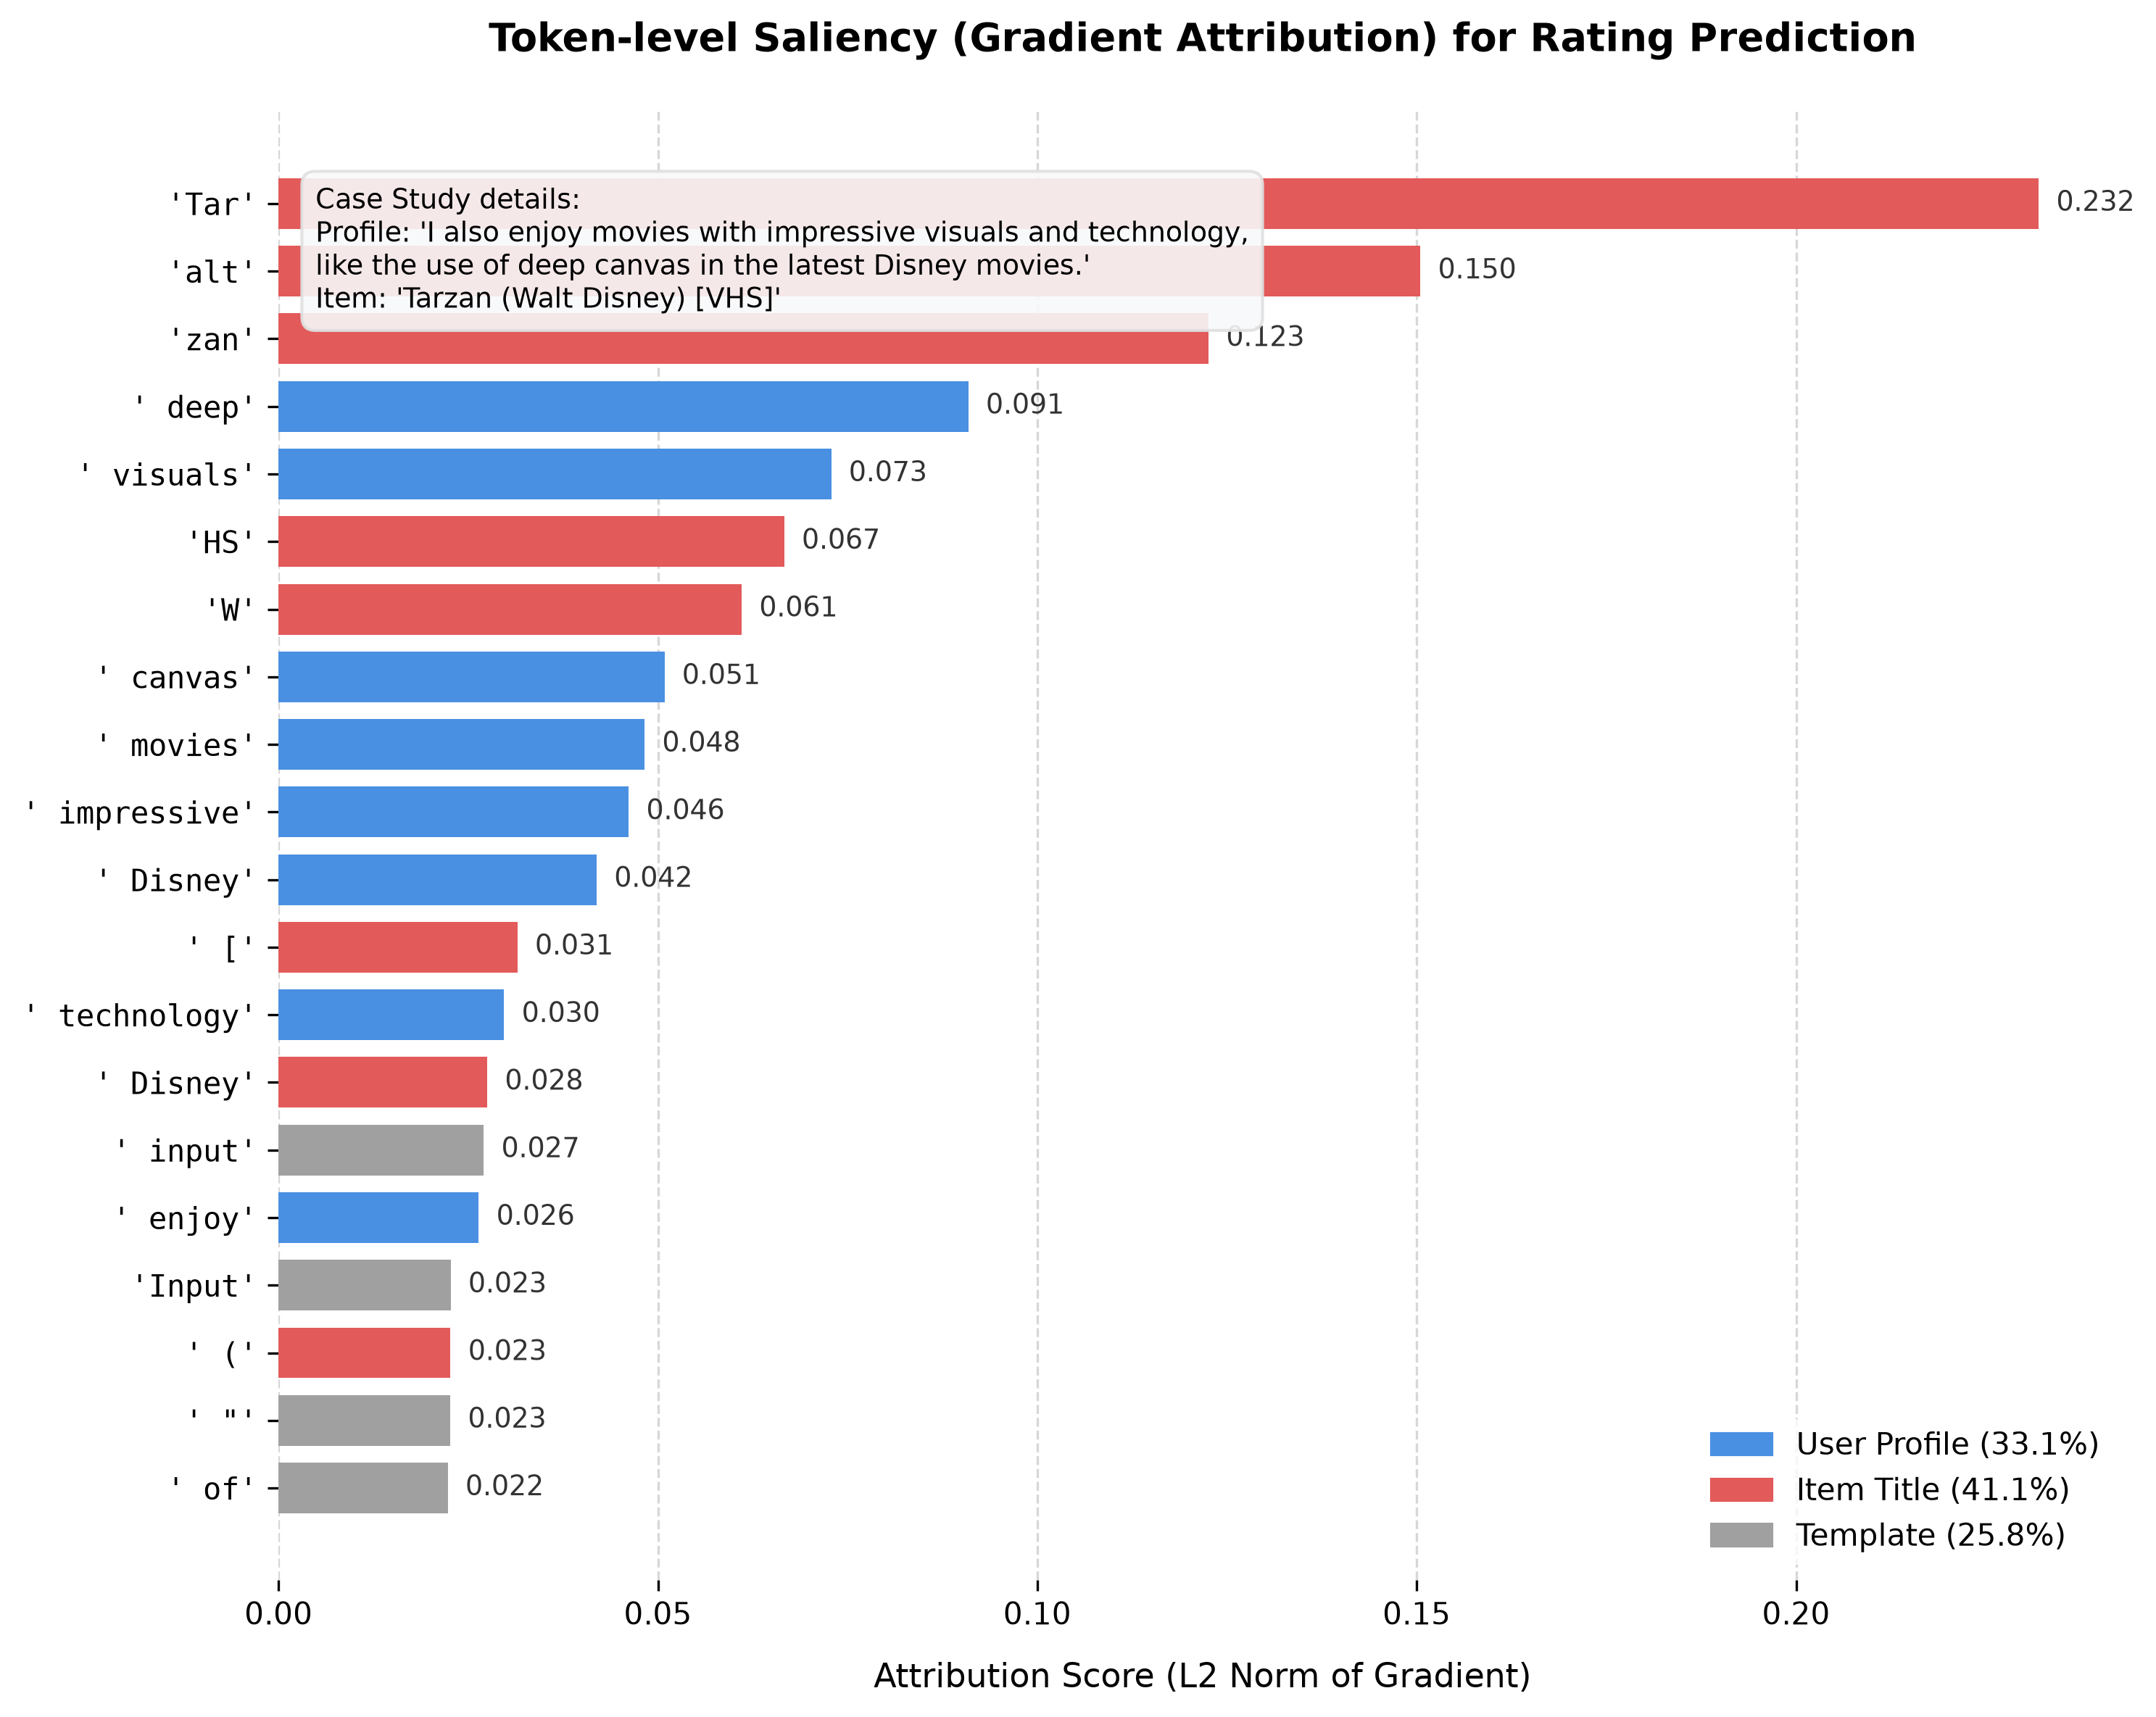
\includegraphics[width=\linewidth]{img/user_profile_attribution.png}
        \caption{\label{fig:attribution}Local feature attribution for a single user profile and target item, as the $L_2$ norm of the input-embedding gradient. See \S\ref{sec:attribution_controls} for controls.}
    \end{minipage}\hfill
    \begin{minipage}{0.48\textwidth}
        \centering
        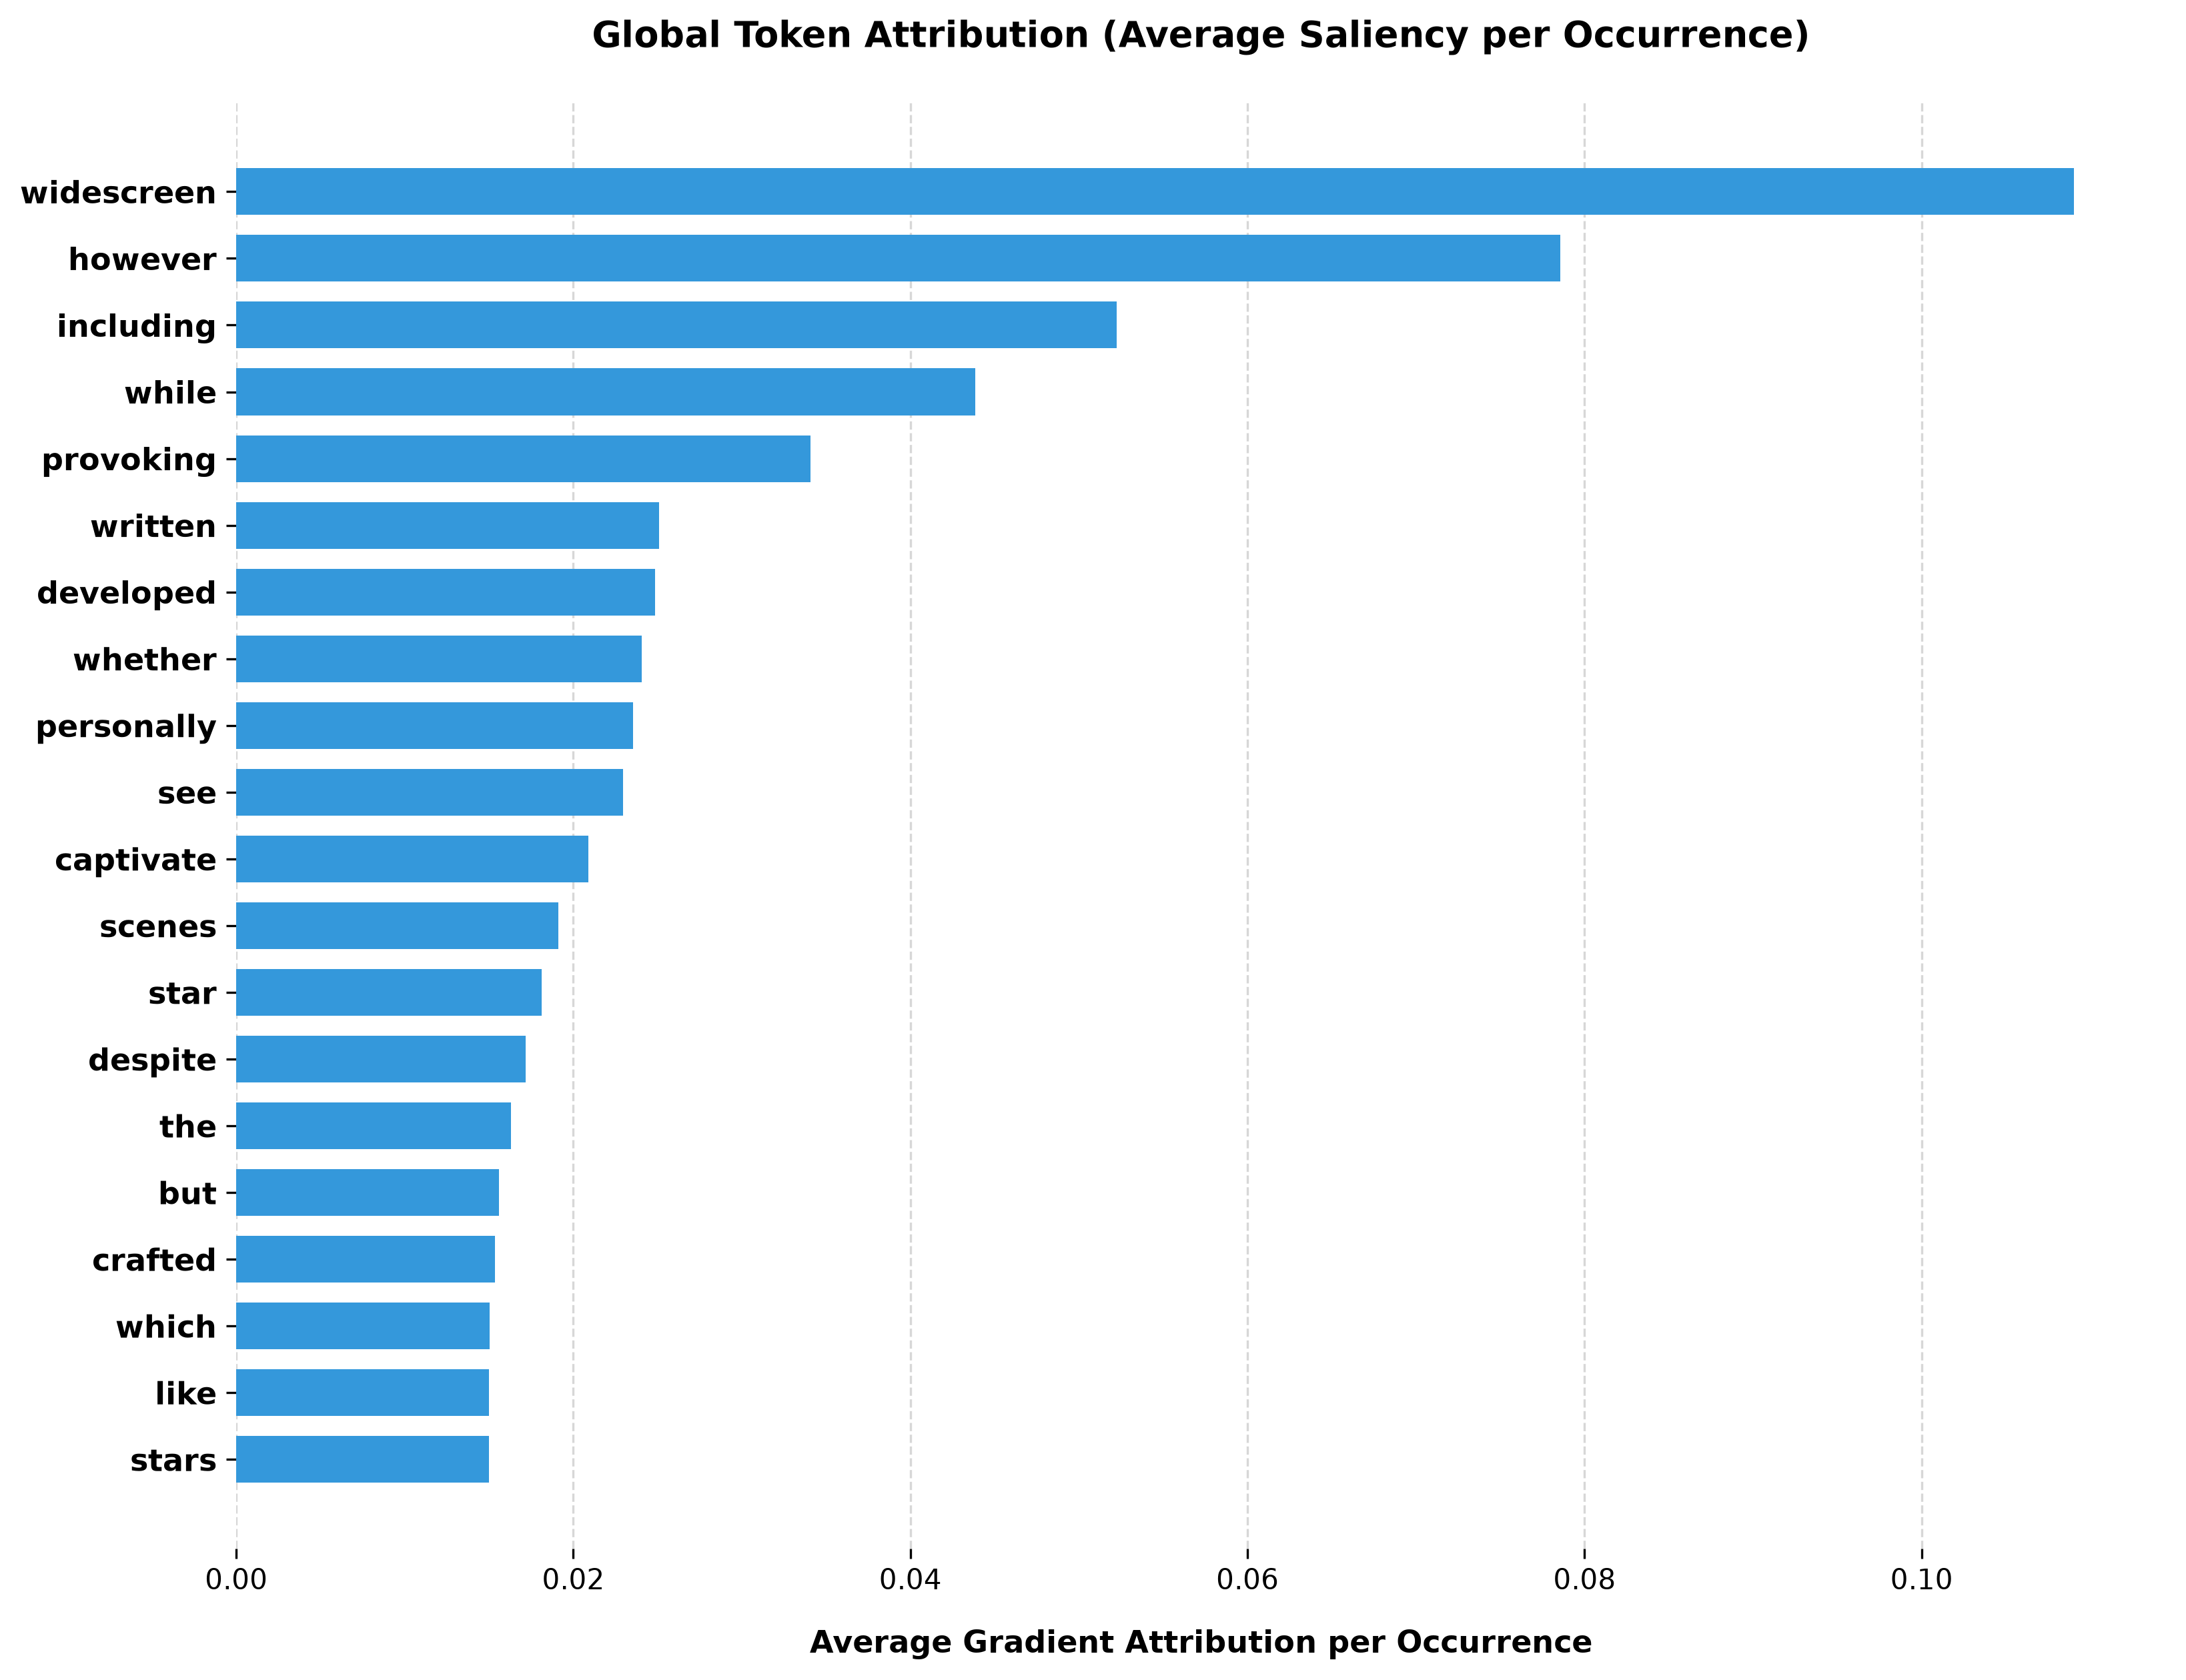
\includegraphics[width=\linewidth]{img/global_profile_attribution.png}
        \caption{\label{fig:global_attribution}Global profile attributions over the Amazon user population. The top terms are dataset artifacts (e.g.\ ``widescreen'') and discourse and style words rather than genre descriptors.}
    \end{minipage}
\end{figure*}

Figures~\ref{fig:attribution} and~\ref{fig:global_attribution} report token-level gradient attribution over profile tokens. Such a pattern could equally reflect the architecture, the pretrained backbone or the profile corpus, so we repeat the global analysis on the pretrained backbone with a randomly initialized head, on the same architecture without pretrained weights, and on word-shuffled profiles, comparing against corpus-frequency and subword-count baselines. Because gradient magnitudes are not comparable across models, we summarize each condition by a scale-invariant statistic: mean attribution on a fixed a-priori genre lexicon divided by mean attribution on all other profile words.

The controls (Table~\ref{tab:attribution_controls}) do not support reading these figures as evidence that fine-tuning concentrates attribution on preference features. Genre words receive roughly \emph{half} the attribution of other profile words (ratio $0.546$, $p{=}0.002$) and none appears in the top $20$, which is led by \texttt{widescreen} alongside discourse and style terms (\texttt{however}, \texttt{while}, \texttt{levity}, \texttt{cinematography}). Eleven of those $20$ recur under random initialization, and attribution correlates at $\rho{=}0.807$ with the fine-tuned model on word-shuffled profiles, so the pattern follows which words are present rather than their arrangement or meaning. Attribution is also negatively correlated with corpus frequency ($\rho{=}-0.320$, $p{=}0.027$), tracking word rarity, while subword count is not a significant driver ($\rho{=}0.212$, $n.s.$). We therefore treat these figures as descriptive of the saliency method and do not claim they isolate features acquired through fine-tuning.

Profile edits thus move the model's representation but not its recommendations, and scrutability in this formulation gives a user control over how generously they are modeled rather than over what they are recommended. Training the same interface against a ranking objective with negative sampling is the change most likely to make profile edits behaviorally meaningful.

% ---------------------------------------------------------------------------------------
% APPENDIX CANDIDATES
%
% Both tables are referenced above but their key numbers are quoted in the prose, so either
% can move to the appendix. If space allows, Table~\ref{tab:steering} is worth keeping in
% the section: it carries the strongest claim, that a full latent reversal leaves rankings
% unchanged. If the attribution subsection moves, take Figures~\ref{fig:attribution}
% and~\ref{fig:global_attribution} with it.
% ---------------------------------------------------------------------------------------

\begin{table}[t]
    \centering
    \small
    \caption{Activation steering at block 6. Adding $\alpha\mathbf{d}$ to the residual stream at the profile token positions, with $\mathbf{d}$ the crime-minus-romance difference of means, drives the probe readout across its full range while leaving ratings and rankings effectively unchanged. Blocks 2 and 9 behave identically. Rank is over the $330$-item set of Table~\ref{tab:behavioral_validation}.}
    \label{tab:steering}
    \begin{tabular}{lccccc}
    \toprule
    & \multicolumn{2}{c}{\textbf{Probe readout}} & \multicolumn{2}{c}{\textbf{Mean $\hat{r}$}} & \textbf{Crime} \\
    \cmidrule(lr){2-3} \cmidrule(lr){4-5}
    $\alpha$ & $P(\text{crime})$ & $P(\text{romance})$ & Crime & Romance & \textbf{rank} \\
    \midrule
    $0$ & 0.064 & 0.934 & 3.999 & 4.096 & 176.9 \\
    $1$ & 0.547 & 0.451 & 3.997 & 4.093 & 176.8 \\
    $2$ & 0.952 & 0.047 & 3.995 & 4.091 & 176.8 \\
    $4$ & 1.000 & 0.000 & 3.991 & 4.088 & 176.8 \\
    $8$ & 1.000 & 0.000 & 3.984 & 4.082 & 176.8 \\
    \bottomrule
    \end{tabular}
\end{table}

\begin{table}[t]
    \centering
    \small
    \caption{Controls for the global attribution analysis. The genre ratio is mean attribution on a fixed genre lexicon over mean attribution on all other profile words ($1.0$ = no distinction). Agreement is the Spearman correlation of per-word attribution with the fine-tuned condition. Genre words are \emph{under}-attributed, and the pattern largely survives removing fine-tuning, removing pretraining, and shuffling word order.}
    \label{tab:attribution_controls}
    \begin{tabular}{lccc}
    \toprule
    \textbf{Condition} & \textbf{Genre ratio} & \textbf{Agreement} $\rho$ & \textbf{Top-20 overlap} \\
    \midrule
    Fine-tuned (reported)      & $0.546$ & ---      & --- \\
    Pretrained backbone only   & $0.381$ & $+0.452$ & $11/20$ \\
    Random initialization      & $1.169$ & $+0.229$ & $11/20$ \\
    Fine-tuned, shuffled words & $1.121$ & $+0.807$ & $10/20$ \\
    \bottomrule
    \multicolumn{4}{l}{\footnotesize vs corpus frequency: $\rho{=}-0.320$ ($p{=}0.027$); vs subword count: $\rho{=}0.212$ ($n.s.$).}
    \end{tabular}
\end{table}
